\documentclass{beamer}
\usetheme{Boadilla}
\usepackage[thinc]{esdiff}
\usepackage{siunitx}
\usepackage{booktabs}
\usepackage{xcolor}
\usepackage{transparent}
\usepackage{graphicx}
\usepackage{subcaption}
\usepackage{tikz}
\usepackage[x11names]{xcolor}

\setbeamertemplate{bibliography item}[text]
\bibliographystyle{apalike}
\newcommand{\backupbegin}{
   \newcounter{finalframe}
   \setcounter{finalframe}{\value{framenumber}}
}
\newcommand{\backupend}{
   \setcounter{framenumber}{\value{finalframe}}
}


\setbeamertemplate{frametitle}[default][center]

\subtitle{}
\title{}
%\titlegraphic{\includegraphics[width=0.9\linewidth,height=0.4\linewidth]{image.png}}
\author{Ole Merkes}
\institute{University of Hamburg}
\date{09.12.2025}


\AtBeginSection[]
{
    \begin{frame}
        %\frametitle{Table of Contents}
        \tableofcontents[currentsection,currentsubsection]
    \end{frame}
}

\begin{document}

% \setbeamertemplate{background canvas}{
% \transparent{0.4}\includegraphics[width=\paperwidth,height=\paperheight]{image.png}
% }%
\begin{frame}
    \titlepage
\end{frame}
%\setbeamertemplate{background canvas}[default]

\begin{frame}
    \frametitle{SML depth}
    \begin{figure}
        \centering
        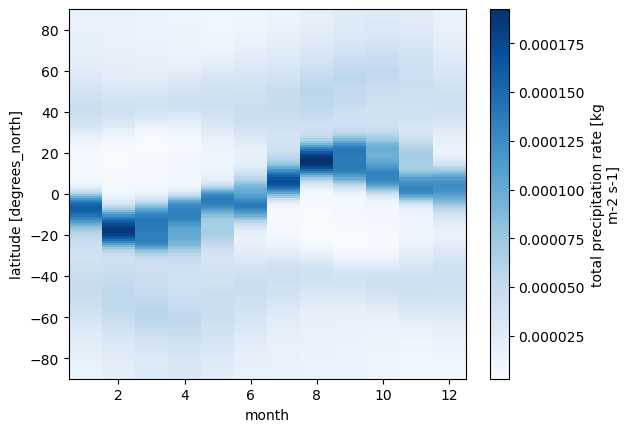
\includegraphics[width=0.9\textwidth]{figures/sml_depth.png}
    \end{figure}
\end{frame}

\begin{frame}
    \frametitle{Spin up}
    \begin{figure}
        \centering
        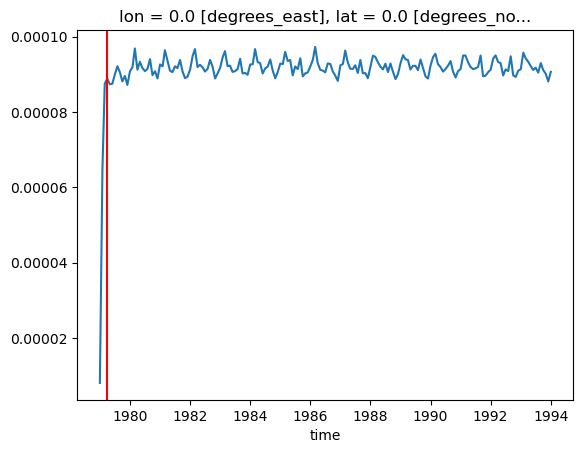
\includegraphics[width=0.8\textwidth]{figures/spin_up.png}
    \end{figure}
\end{frame}

\begin{frame}
    \frametitle{Scaling of the HC}
    \begin{block}{Angular momentum conserving}
        
    \begin{align}
        \Phi_H\sim&\left(\frac{gH\Delta_h}{\Omega^2R_E^2}\right)^{1/2}\\
        \psi_\mathrm{max} \sim & \frac{1}{\tau}\frac{g^{3/2}(H\Delta_h)^{5/2}}{\Omega^3R_E^2\Delta_v}
    \end{align}
    \end{block}
    \begin{block}{Baroclinic instability}
        \begin{align}
            \theta_C \sim \left(\frac{NH}{2\Omega a}\right)^{1/2}
        \end{align}
    \end{block}
\end{frame}

\begin{frame}
    \frametitle{4x CO2}
    \begin{itemize}
        \item global warming: tropopause height
        and stability increase while meridional
        temperature gradient in the subtropical
        atmosphere decreases
    \end{itemize}
\end{frame}

\begin{frame}
    \frametitle{Research gap?}
    \begin{itemize}
        \item D’Agostino, R., P. Lionello, O. Adam,
and T. Schneider (2017), Factors
controlling Hadley circulation changes
from the Last Glacial Maximum
to the end of the 21st century,
Geophys. Res. Lett., 44, 8585–8591,
doi:10.1002/2017GL074533.
        \end{itemize}
\end{frame}
\begin{frame}
    \frametitle{Research gap?}
    \begin{columns}
    \begin{column}{0.3\textwidth}
        \begin{itemize}
            \item PMIP3 and CMIP5 data from the Last Glacial Maximum (LGM), Mid-Holocene (MIDH),
            Pre-Industrial Control (PIC), Historical (HIST), and Representative Concentration Pathways 4.5 and 8.5 experiments
        \end{itemize}
    \end{column}
    \begin{column}{0.7\textwidth}  %%<--- here
    \begin{center}
        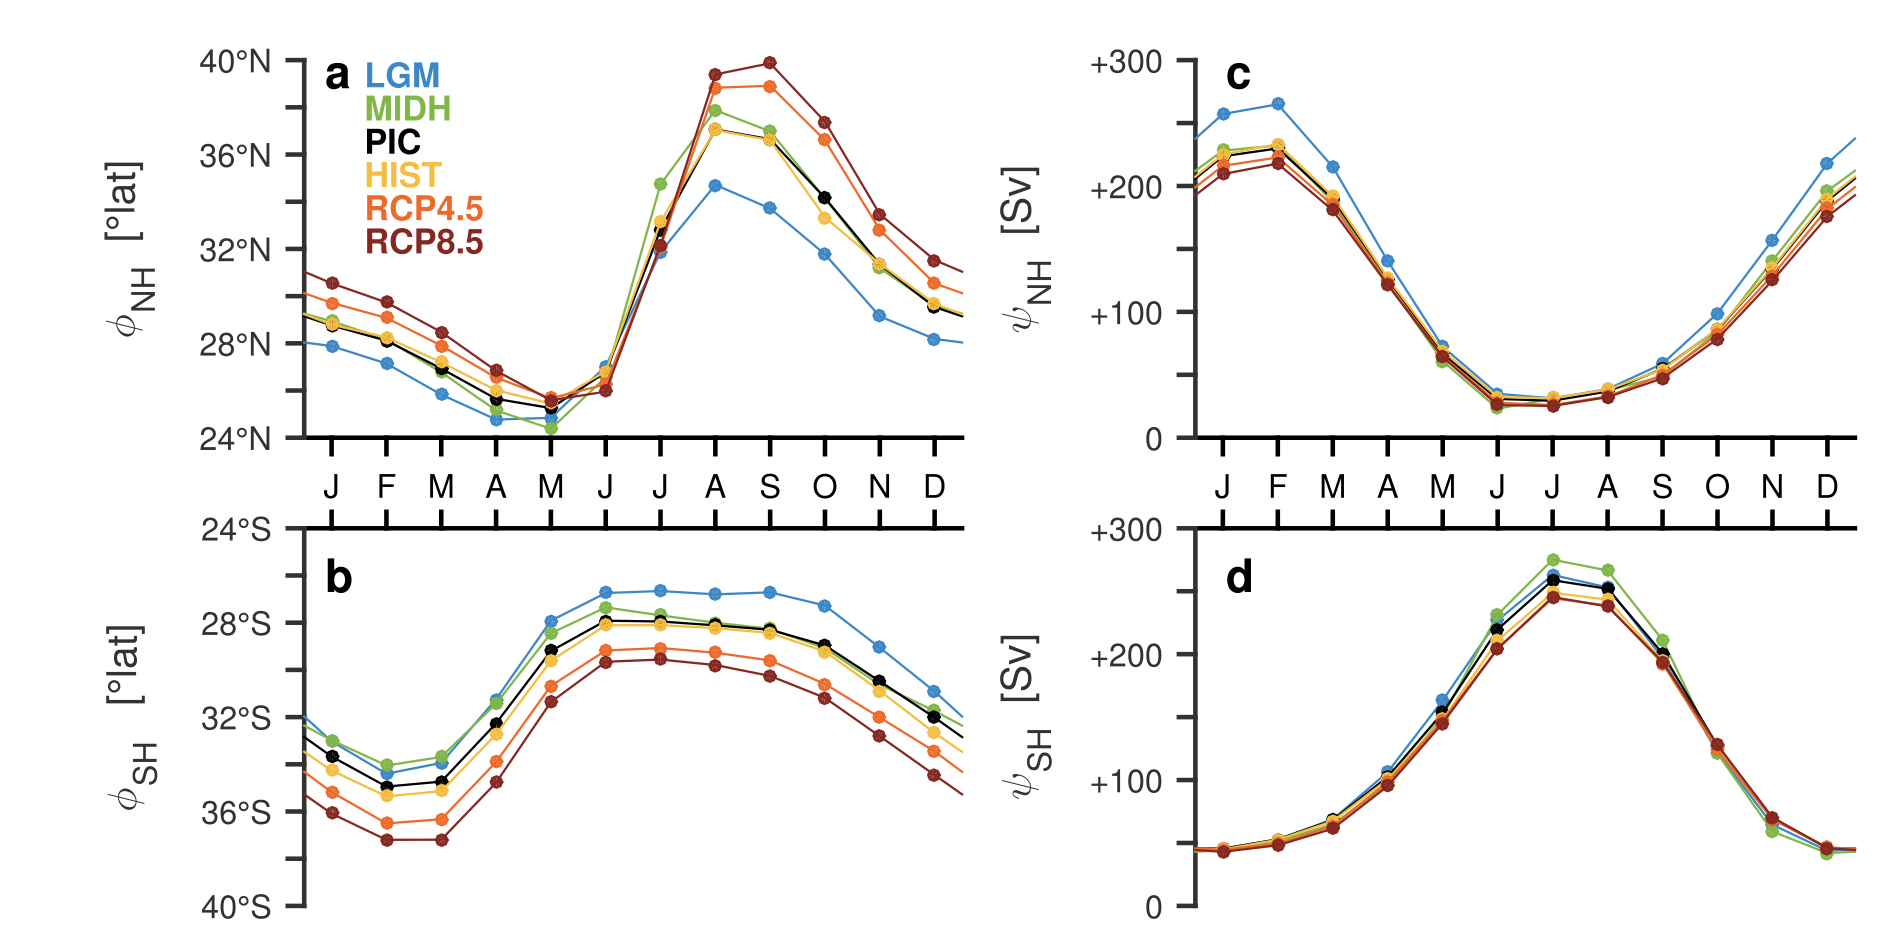
\includegraphics[width=1.0\textwidth]{figures/HC_variability.png}
    \end{center}
\end{column}
\end{columns}
\end{frame}

\begin{frame}
    \frametitle{Research gap?}
    \begin{columns}
    \begin{column}{0.3\textwidth}
    Multimodel ensemble mean stream function difference between LGM, MIDH, and RCP8.5 and relative to PIC    \end{column}
    \begin{column}{0.7\textwidth}  %%<--- here
    \begin{center}
        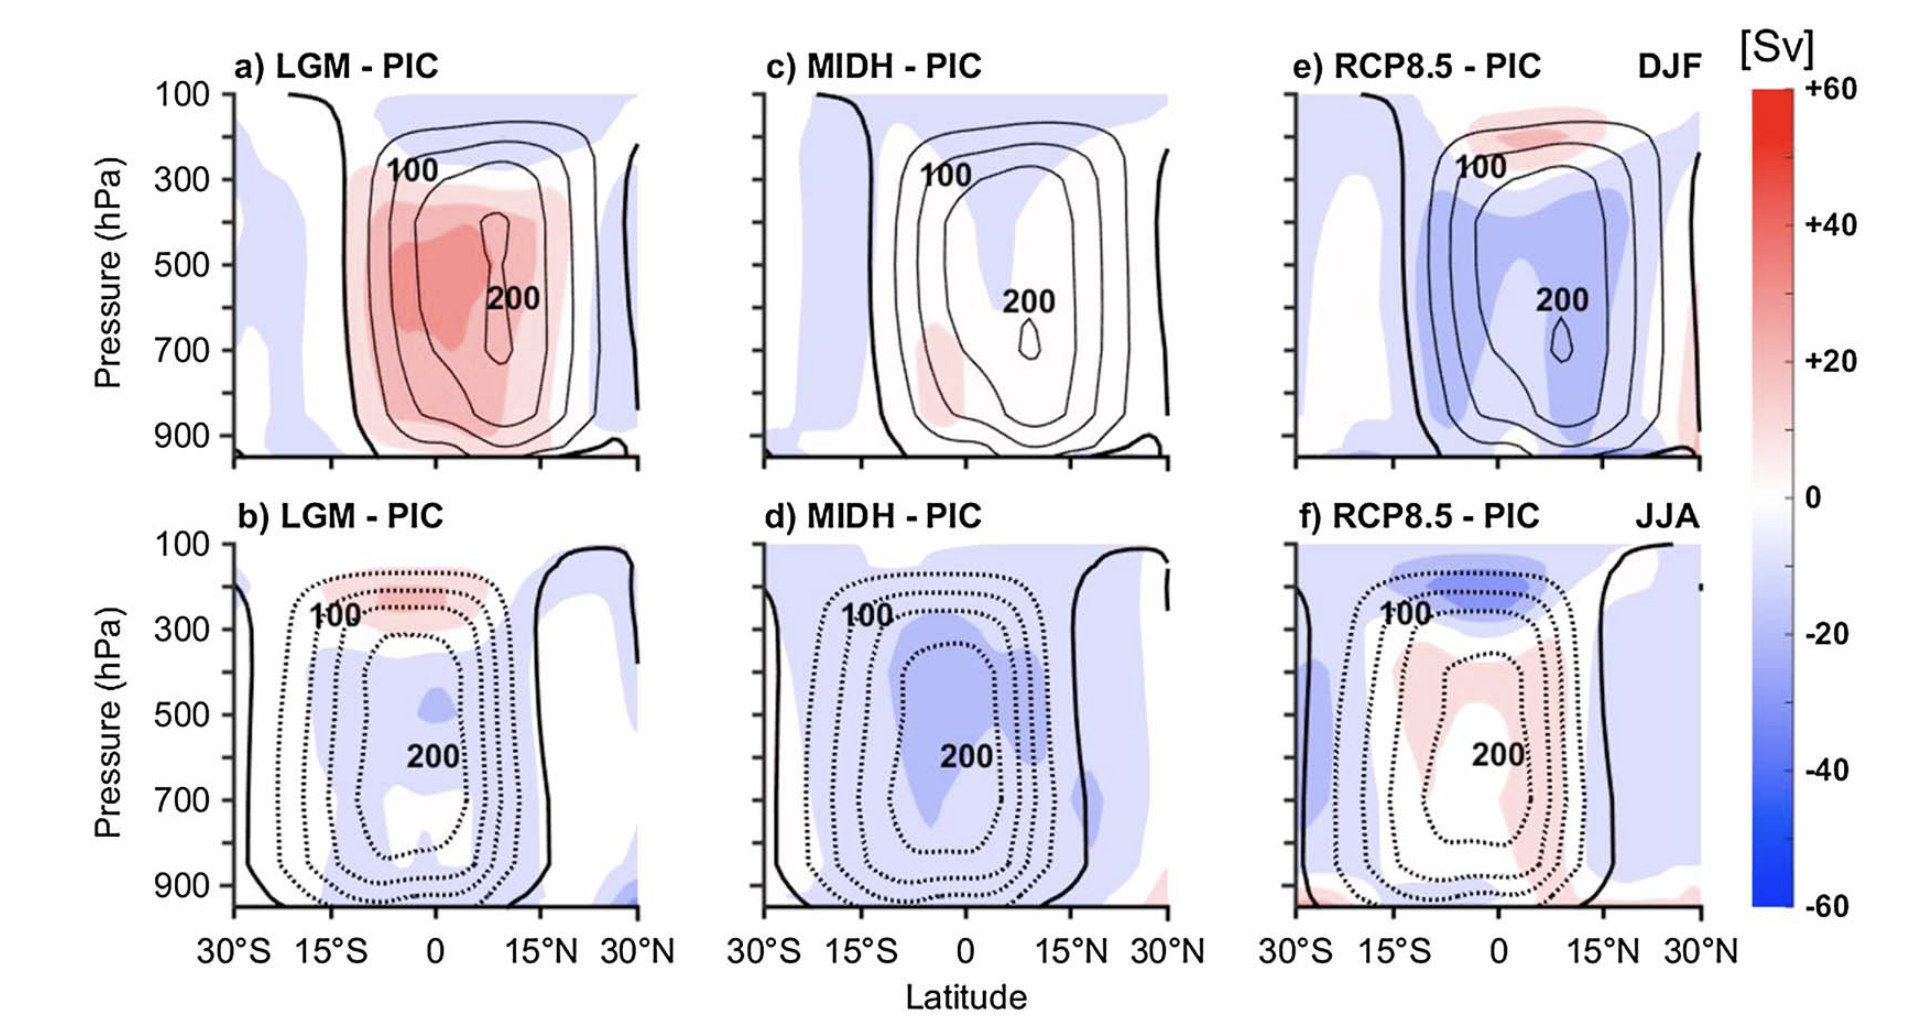
\includegraphics[width=1.0\textwidth]{figures/HC_structure.png}
    \end{center}
\end{column}
\end{columns}
\end{frame}
\backupbegin

\backupend
\end{document}
